\section{Grundlagen des Aufbaus}
\subsection{Node Editor}
\begin{figure}[h]
    \centering
    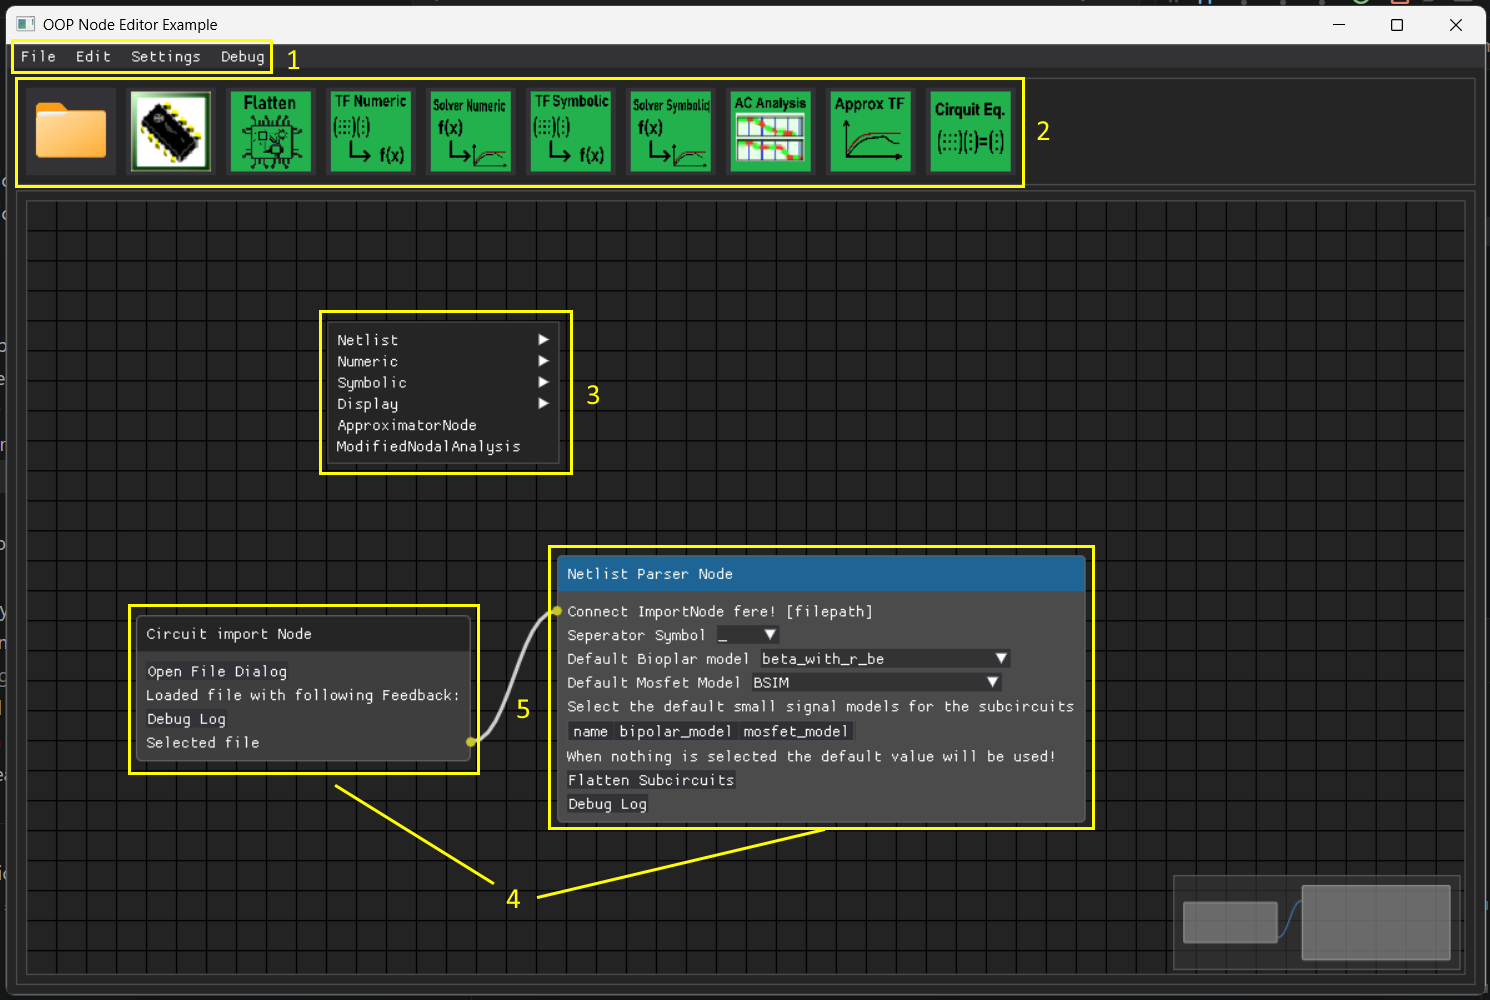
\includegraphics[width=0.8\textwidth]{bilder/window_node-editor.png}
    \caption{Aufbau des Node-Editors}
    \label{fig:window_node-editor}
\end{figure}

Der Node-Editor ist in folgende Bereiche Aufgeteilt.

\textbf{Menüleiste (1)} \\
Über diese Menuleiste kann der gesamte NodeEditor gespeichert und geladen werden, Einstellungen getroffen werden und Knoten eingefügt werden.

\textbf{Schnellleiste für das Einfügen von Knoten (2)} \\
\label{layout_schnellleiste}
Über die Schnelleiste können schneller Knoten eingefügt werden. Wenn ein Knoten ausgewählt oder bearbeitet wurde kann über die Schnelleiste leicht ein folge-Knoten eingefügt werden. Dieser wird dann automatisch mit dem vorherigen Knote verbunden. Es können nur die Knoten angeklickt werden, welche mit dem verherigen Knoten verbunden werden können.

\textbf{Rechtsklick-Menu zum einfügen von Knoten (3)} \\
\label{layout_rightclick_add_node}
Mit einem Rechtsklick auf den Hintergrund öffnet sich an der Mausposition ein Menu zum einfügen eines Knoten. Der Knoten erscheint an der selben Position wie das Menu.

\textbf{Knoten (4)} \\
Zwei eingefügte Knoten. Diese können verschoben werden. Ausgewählte Knoten können mit der Entfernen Taste gelöscht werden.

\textbf{Verlinkung zwischen Knoten (5)} \\
Eine Verbindung zwischen zwei Knoten. Verbindungen können über Strg+Linksklick entfernt werden. Knotenverbindungen werden zwischen den Input- und Output Pins erstellt (Punkte an dem Knoten)

\subsection{Mögliche Einstellungen}
\subsubsection{Design}
Die Darstellung des Programms / Das Design kann über das Fenster-Menu, unter dem Menupunkt Settings->StyleEditor eingestellt werden.

\begin{figure}[h]
    \centering
    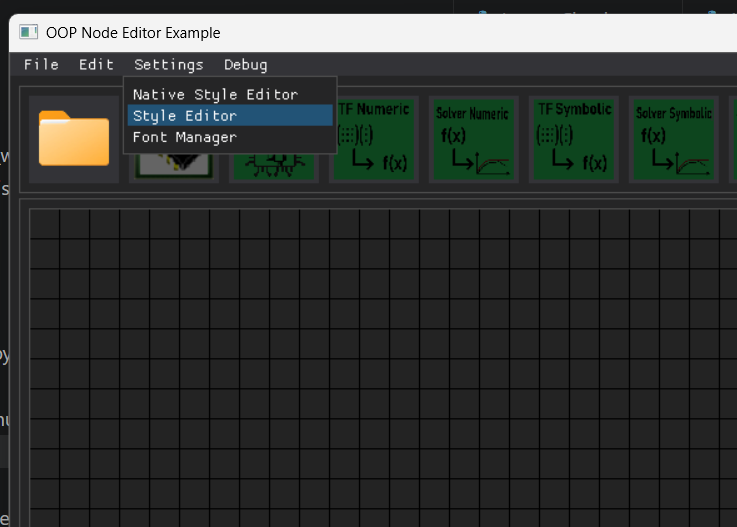
\includegraphics[width=0.8\textwidth]{bilder/setting_design.png}
    \caption{Auswahl des Style-Editors im Fenster Menu}
    \label{fig:settings_style-editor}
\end{figure}

\begin{figure}[h]
    \centering
    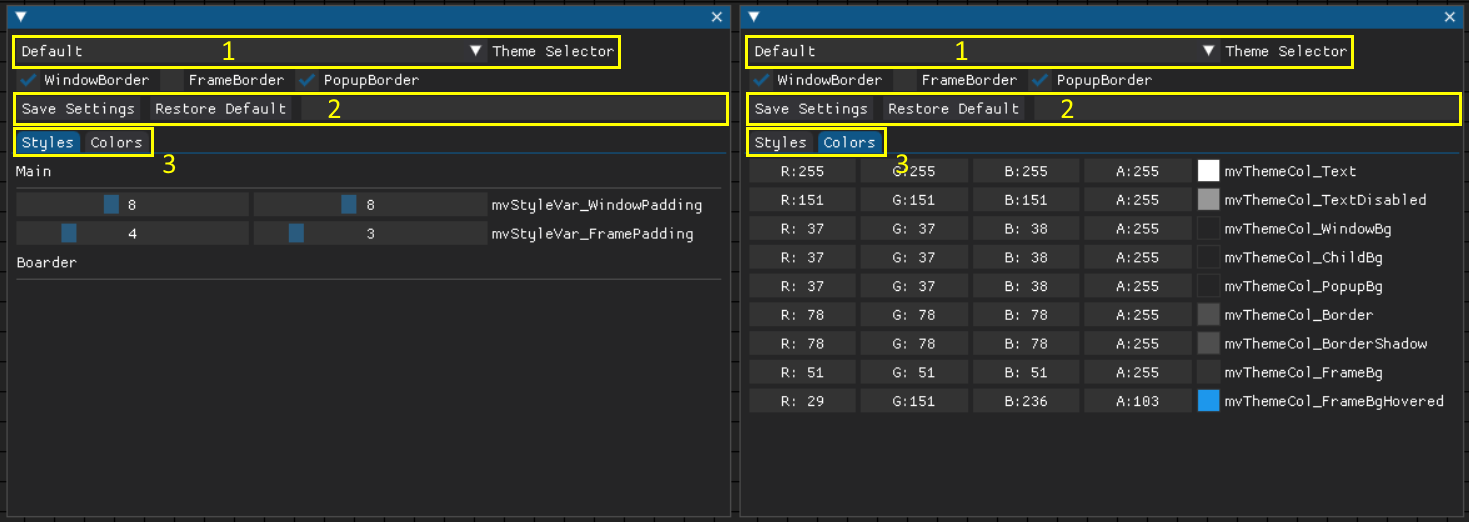
\includegraphics[width=0.8\textwidth]{bilder/settings_style-editor.png}
    \caption{Aufbau des Style Editors}
    \label{fig:window_style-editor}
\end{figure}

Im der \autoref{fig:window_style-editor} kann man den Aufbau des Style-Editors sehen. Der erste Bereich besteht aus einem Dropdownmenu mit welchen ein gespeichertes Design ausgewählt werden kann.\\
Ein eigenes Design kann mit den Einstellungen unter Bereich 3 erstellt werden. Fertige Designs können können unter dem Knopf: \enquote{Save Settings} und dem dem davon rechts liegenden Textfeld gespeichert werden. Zuerst muss der Name des Designs im rechten Textfeld eingegeben werden.